\documentclass[border=5pt]{standalone}
\usepackage[T1]{fontenc}
\RequirePackage[semibold]{sourcesanspro}
\usepackage{pgfplots}
\usepackage{xcolor}
\usepackage{caption}

\captionsetup{
  font={
    footnotesize,
    sf,
%    sansmath
  },
  labelfont=bf,
  labelsep=period
}

\pgfplotsset{compat=1.18}

% Define colors
\definecolor{fullmodel}{HTML}{2171B5}
\definecolor{ablated}{HTML}{E0E0E0}
\definecolor{baseline}{HTML}{EF6C00}
\definecolor{random}{HTML}{BDBDBD}
\definecolor{textgray}{HTML}{404040}
\definecolor{deltagray}{HTML}{888888}

\begin{document}
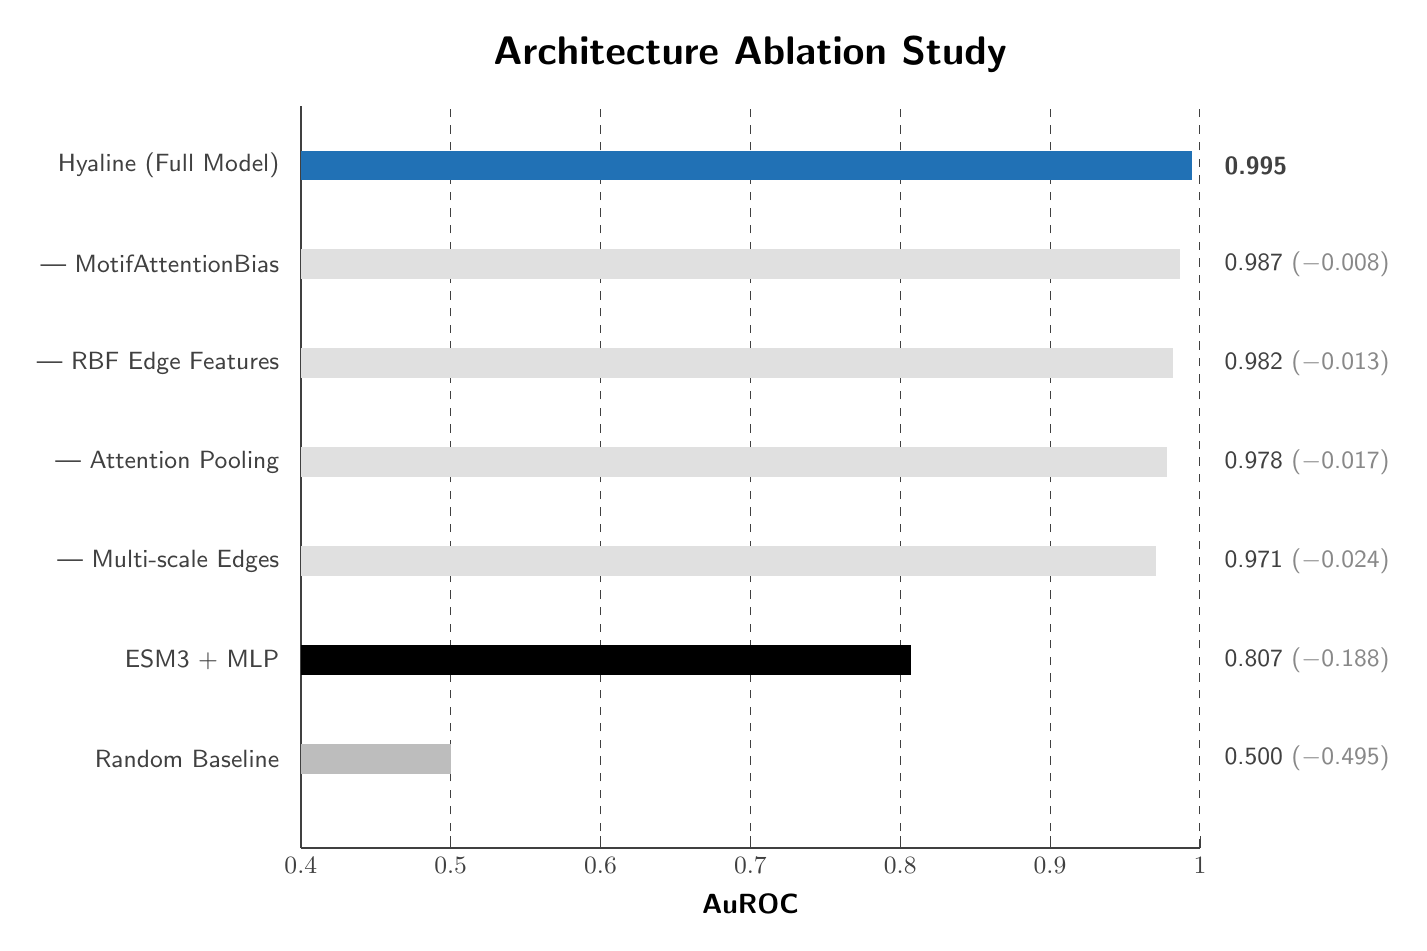
\begin{tikzpicture}

\begin{axis}[
    font=\footnotesize\sffamily,
    % Chart dimensions - taller for more spacing
    width=13cm,
    height=11cm,
    % Horizontal bar chart
    xbar,
    bar width=18pt,
    % Axis settings
    xmin=0.4,
    xmax=1.0,
    ymin=-0.5,
    ymax=6.2,
    % Y-axis labels
    ytick={0,1,2,3,4,5,6},
    yticklabels={
        {Random Baseline},
        {ESM3 + MLP},
        {--- Multi-scale Edges},
        {--- Attention Pooling},
        {--- RBF Edge Features},
        {--- MotifAttentionBias},
        {Hyaline (Full Model)}
    },
    y tick label style={
        font=\small\sffamily,
        color=textgray,
        anchor=east,
        align=right,
    },
    % X-axis settings
    xlabel={\textbf{AuROC}},
    xlabel style={font=\normalsize\sffamily, at={(0.5,-0.05)}},
    xtick={0.4, 0.5, 0.6, 0.7, 0.8, 0.9, 1.0},
    xticklabel style={font=\small\sffamily, color=textgray},
    % Title
    title={\Large\textbf{Architecture Ablation Study}},
    title style={at={(0.5,1.01)}},
    % Grid and axis styling
    axis line style={textgray, line width=0.6pt},
    tick style={textgray},
    ytick style={draw=none},
    % Axis lines
    axis x line*=bottom,
    axis y line*=left,
    % Add subtle grid
    xmajorgrids=true,
    grid style={textgray, line width=0.3pt, dashed},
    % Clip settings
    clip=false,
    % Enlarge limits
    enlarge y limits={abs=0.4},
]

% Draw bars manually using fill between or nodes
% Random Baseline (light gray) - y=0
\fill[random] (axis cs:0.4,0-0.15) rectangle (axis cs:0.500,0+0.15);

% ESM3 + MLP (orange) - y=1
\fill[baseline] (axis cs:0.4,1-0.15) rectangle (axis cs:0.807,1+0.15);

% Ablated models (dark gray)
\fill[ablated] (axis cs:0.4,2-0.15) rectangle (axis cs:0.971,2+0.15);
\fill[ablated] (axis cs:0.4,3-0.15) rectangle (axis cs:0.978,3+0.15);
\fill[ablated] (axis cs:0.4,4-0.15) rectangle (axis cs:0.982,4+0.15);
\fill[ablated] (axis cs:0.4,5-0.15) rectangle (axis cs:0.987,5+0.15);

% Full model (blue) - y=6
\fill[fullmodel] (axis cs:0.4,6-0.15) rectangle (axis cs:0.995,6+0.15);

% Add value labels - all on the right side
\node[anchor=west, font=\small\sffamily\bfseries, color=textgray] at (axis cs:1.01,6) {0.995};
\node[anchor=west, font=\small\sffamily, color=textgray] at (axis cs:1.01,5) {0.987 {\color{deltagray}($-$0.008)}};
\node[anchor=west, font=\small\sffamily, color=textgray] at (axis cs:1.01,4) {0.982 {\color{deltagray}($-$0.013)}};
\node[anchor=west, font=\small\sffamily, color=textgray] at (axis cs:1.01,3) {0.978 {\color{deltagray}($-$0.017)}};
\node[anchor=west, font=\small\sffamily, color=textgray] at (axis cs:1.01,2) {0.971 {\color{deltagray}($-$0.024)}};
\node[anchor=west, font=\small\sffamily, color=textgray] at (axis cs:1.01,1) {0.807 {\color{deltagray}($-$0.188)}};
\node[anchor=west, font=\small\sffamily, color=textgray] at (axis cs:1.01,0) {0.500 {\color{deltagray}($-$0.495)}};

\end{axis}

\end{tikzpicture}
\end{document}